First, we created an U-Net\cite{unet} model for semantic segmentation based on images Gleason pattern(GP) of prostate pathological images. The labels are normal glands, GP3, GP4, and GP5. We use VGG16\cite{vgg} for the ecoder part of the U-Net model and nearest sampling for the decoder part.\par

\vspace{0.5zh}

The model was trained by whole slide image of total prostatectomy specimens diagnosed in our department and those labels like Fig\ref{fig:seg_color}. An example output of the model is shown in Fig\ref{fig:dl_sample}. \par

\vspace{-1zh}

\begin{figure}[htbp]\centering
  \begin{tabular}{c}
    \begin{subfigure}[t]{0.20\columnwidth}\centering
      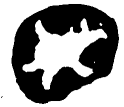
\includegraphics[width=0.7\columnwidth]{assets/gp_pin.png}
      \subcaption{Normal gland:black}
    \end{subfigure}

    \begin{subfigure}[t]{0.15\columnwidth}\centering
      
\includegraphics[width=0.7\columnwidth]{assets/gp_3_2.png}
      \subcaption{GP3:blue}
    \end{subfigure}

    \begin{subfigure}[t]{0.15\columnwidth}\centering
      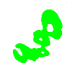
\includegraphics[width=0.7\columnwidth]{assets/gp_4.png}
      \subcaption{GP4:green}
    \end{subfigure}

    \begin{subfigure}[t]{0.15\columnwidth}\centering
      
\includegraphics[width=0.7\columnwidth]{assets/gp_5_2.png}
      \subcaption{GP5:red}
    \end{subfigure}

    \begin{subfigure}[t]{0.15\columnwidth}\centering
      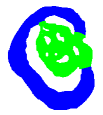
\includegraphics[width=0.7\columnwidth]{assets/gp_3_1.png}
      \subcaption{GP3+4}
    \end{subfigure}

    \begin{subfigure}[t]{0.15\columnwidth}\centering
      
\includegraphics[width=0.7\columnwidth]{assets/gp_5_1.png}
      \subcaption{GP4+5}
    \end{subfigure}
  \end{tabular}
  \label{fig:example}
  \caption{Example of the segmentation}
  \label{fig:seg_color}
\end{figure}

\begin{figure}[htbp]\centering
  \begin{tabular}{c}
    \begin{subfigure}[t]{0.33\columnwidth}\centering
      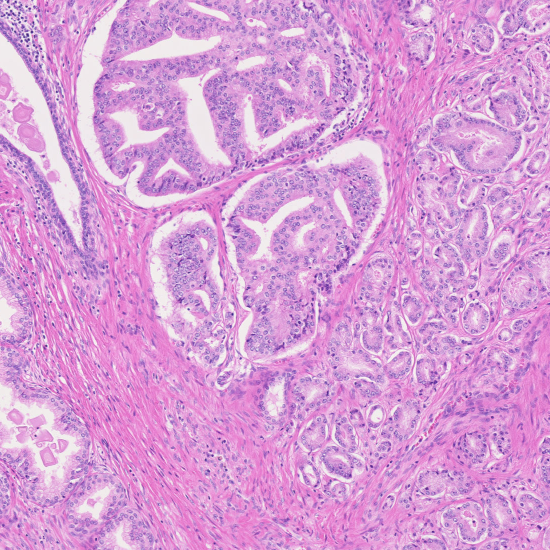
\includegraphics[width=0.9\columnwidth]{assets/ex_org.png}
      \subcaption{Input image}
    \end{subfigure}

    \begin{subfigure}[t]{0.33\columnwidth}\centering
      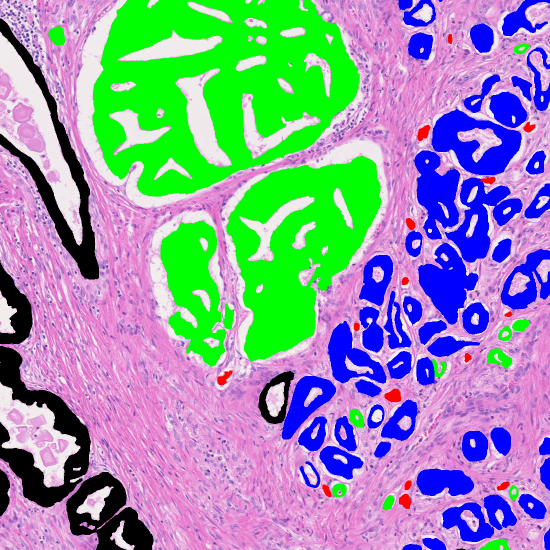
\includegraphics[width=0.9\columnwidth]{assets/ex_gt.png}
      \subcaption{Label image}
    \end{subfigure}

    \begin{subfigure}[t]{0.33\columnwidth}\centering
      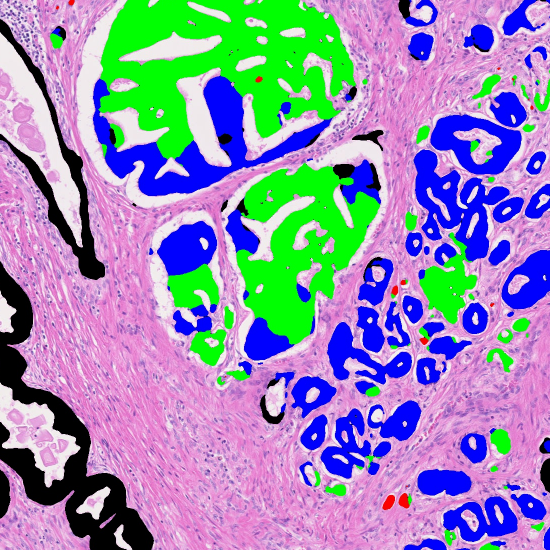
\includegraphics[width=0.9\columnwidth]{assets/ex_pr.png}
      \subcaption{Output image}
    \end{subfigure}
  \end{tabular}
  \label{fig:example}
  \caption{Example output ofr the U-Net model}
  \label{fig:dl_sample}
\end{figure}

The IoU (Intersection over union) calculated by the Jaccard index of the U-Net model were 0.765 for the training datasets and 0.737 for the testing datasets.

\begin{align}
  \label{eq:iou}
  Jaccard\,index = & \; \frac{|PR \cap GT|}{|PR \cup GT|} \\[5mm]
  PR: \mbox{Prediction} & \;\; GT: \mbox{Ground truth} \nonumber
\end{align}

\vspace{0.5zh}

In addition, we developed the client/server applications(Fig\ref{fig:arch}). The client gets the images from the microscopic camera, sends to the server via HTTP and displays the results. It is installed into Raspberry Pi 4 Model B. The server receives the images, passes them to the DL system and serves the results. It is into the computer where DL system works.\par

\vspace{1zh}

\begin{figure}\centering
  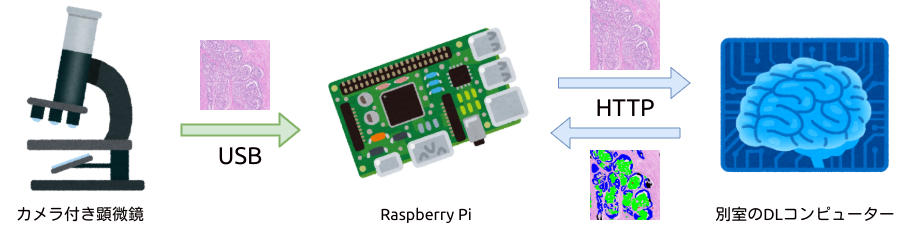
\includegraphics[width=\columnwidth]{assets/arch.png}
  \caption{Architecture of client and server applications}
  \label{fig:arch}
\end{figure}

The DL system and the client/server applications were all written in Python and work on Linux-based computers. Especially the DL system uses PyTorch and the client uses GTK+/GStreamer. The source codes are all available on GitHub.\cite{gh-prostate}\cite{gh-pai} \par
